\documentclass{standalone}
\usepackage{PhysicalChemistryNote}
\begin{document}
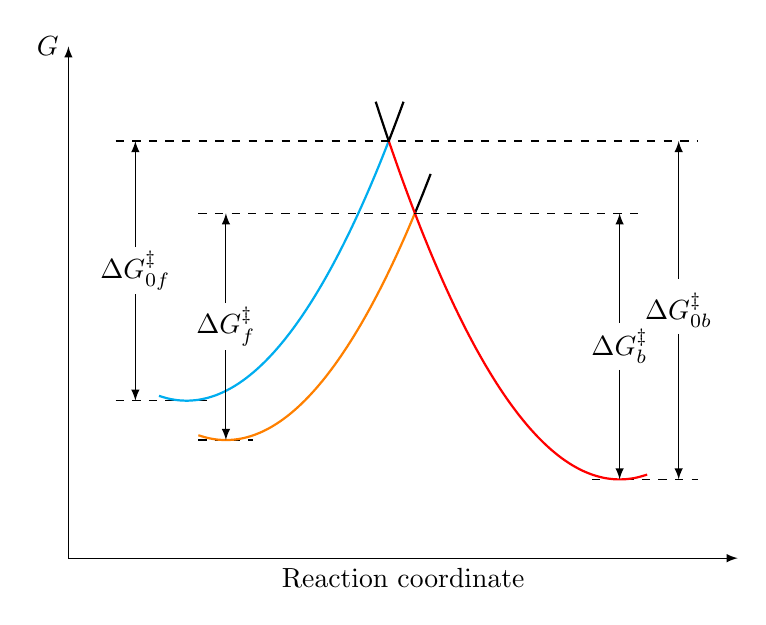
\begin{tikzpicture}
    \draw[-latex] (-1,0)--(7.5,0);
    \node[below] at (3.25,0) {Reaction coordinate};
    \draw[-latex] (-1,0)--(-1,6.5) node[left] {$G$};
    \draw[dashed] (-0.4,2)--(0.85,2);
    \draw[dashed] (0.65,1.5)--(1.35,1.5);
    \draw[dashed] (5.65,1)--(7,1);
    \draw[thick,cyan,domain=0.15:3.068] plot[smooth] (\x,{(\x-0.5)^2/2+2});
    \draw[thick,domain=3.068:3.2557] plot[smooth] (\x,{(\x-0.5)^2/2+2});
    \draw[thick,orange,domain=0.65:3.4] plot[smooth] (\x,{(\x-1)^2/2+1.5});
    \draw[thick,domain=3.4:3.6] plot[smooth] (\x,{(\x-1)^2/2+1.5});
    \draw[thick,red,domain=3.068:6.35] plot[smooth] (\x,{(\x-6)^2/2+1});
    \draw[thick,domain=2.9026:3.068] plot[smooth] (\x,{(\x-6)^2/2+1});
    \draw[dashed] (-0.4,5.29777)--(7,5.29777);
    \draw[dashed] (0.65,4.38)--(6.25,4.38);
    \node at (-0.15,3.6488) {$\Delta G^\ddagger_{0\text f}$};
    \draw[-latex] (-0.15,3.9488)--(-0.15,5.2977);
    \draw[-latex] (-0.15,3.3488)--(-0.15,2);
    \node at (1,2.94) {$\Delta G^\ddagger_{\text f}$};
    \draw[-latex] (1,3.24)--(1,4.38);
    \draw[-latex] (1,2.64)--(1,1.5);
    \node at (6.75,3.1488) {$\Delta G^\ddagger_{0\text b}$};
    \draw[-latex] (6.75,3.5488)--(6.75,5.2977);
    \draw[-latex] (6.75,2.8488)--(6.75,1);
    \node at (6,2.69) {$\Delta G^\ddagger_{\text b}$};
    \draw[-latex] (6,2.99)--(6,4.38);
    \draw[-latex] (6,2.39)--(6,1);
\end{tikzpicture}
\end{document}